\documentclass[aspectratio=169,11pt]{beamer}
\usepackage{assets/restrepo-beamer}
\title[Acemoglu y Restrepo: salarios y automatización]{The Race between Man and Machine}
\subtitle{La condición detrás del efecto salarial}
\author{Belén Vásquez}
\institute{Modelamiento Económico con IA \textperiodcentered{} Universidad del Pacífico}
\date{Septiembre de 2026}
\newcommand{\NBER}{NBER rev. junio 2017}
\begin{document}

% 1 -- 0:30
\begin{frame}[plain]
\titlepage
\vspace{-1em}
\begin{center}\small\href{\RepoURL}{\texttt{github.com/sbvasquezg-ux/ai-06-restrepo}}\end{center}
\sourcefoot{Acemoglu y Restrepo, AER 2018, 108(6), pp. 1488--1542. Trabajo sobre \NBER.}
\end{frame}

% 2 -- 0:45
\begin{frame}{La pregunta exige distinguir tres resultados}
\begin{keybox}\large ¿La automatización reduce \textbf{necesariamente} el salario y la participación laboral?\end{keybox}
\medskip
\begin{itemize}
\item \textbf{Salario real}: $W$, cuánto paga una unidad de trabajo.
\item \textbf{Participación}: $s_L=WL/(RK+WL)$, fracción del producto neto que remunera al trabajo.
\item \textbf{Empleo}: $L$, oferta y uso agregado de trabajo.
\end{itemize}
\medskip
\textbf{Cambio de escala.} Aquí se estudia una economía agregada. Los precios, la oferta laboral y, después, el capital y la innovación se ajustan conjuntamente.
\sourcefoot{\NBER, Prop. 2, pp. 11--12; definición de $s_L$, p. 10, nota 14. Nivel del curso: issue 5.}
\end{frame}

% 3 -- 1:00
\begin{frame}{Tareas factibles y tareas efectivamente automatizadas}
\[
Y=\widetilde B\left[\int_{N-1}^{N}y(i)^{(\sigma-1)/\sigma}\,di\right]^{\sigma/(\sigma-1)}.
\]
\begin{columns}[T,onlytextwidth]
\column{.53\textwidth}
En el límite $\eta\to0$:
\[
y(i)=\begin{cases}k(i)+\gamma(i)l(i),&i\le I,\\\gamma(i)l(i),&i>I.\end{cases}
\]
$\gamma$ positiva y estrictamente creciente. $\sigma>0$ finita; en uno se toma el límite.
\column{.43\textwidth}
\[
I^*=\min\{I,\widetilde I\},\qquad\gamma(\widetilde I)=W/R.
\]
\textbf{Factibilidad}: $I$.\\[.4em]
\textbf{Adopción}: $I^*$.\\[.4em]
\textbf{Tareas de trabajo}: $N-I^*$.
\end{columns}
\medskip
La masa total de tareas es uno: $N$ reemplaza tareas inferiores con nuevas versiones.
\sourcefoot{\NBER, ecs. (1)--(3), pp. 6--7; ec. (6), p. 8. Especialización $\eta\to0$ declarada.}
\end{frame}

% 4 -- 1:00
\begin{frame}{Supuestos que sostienen la estática comparativa}
\small
\begin{tabular}{p{.20\textwidth}p{.72\textwidth}}
\toprule
Hipótesis & Qué permite afirmar \\\midrule
Assumption 1 & Ventaja comparativa estricta: un umbral ordena las tareas.\\[.6em]
Assumption 2 & $\eta\to0$ o $\zeta=1$; demanda homotética y forma cerrada. $s=\widehat\sigma=(1-\eta)\sigma+\eta\zeta$.\\[.6em]
Assumption 3 & $K<\overline K$, con $R>W/\gamma(N)$: nuevas tareas rentables.\\[.6em]
Preferencias (4) & $L=L^s(\omega)$ creciente, $\omega=W/(RK)$ y $\varepsilon_L>0$.\\[.6em]
Interioridad & $K$ fijo, $N-1<I^*=I<\widetilde I$; $W,R>0$ y $0<s_L<1$.\\\bottomrule
\end{tabular}
\medskip
Las derivadas son \textbf{locales}. Cambiar de régimen requiere otro argumento.
\sourcefoot{\NBER, Assumptions 1--3 y ec. (4), pp. 7--8; ec. (11), p. 10; Props. 2--3, pp. 11--13.}
\end{frame}

% 5 -- 1:00
\begin{frame}{Participación y empleo caen; el salario es ambiguo}
\begin{center}
\begin{tabular}{lccc}
\toprule
Experimento local & $W$ & $s_L$ & $L$\\\midrule
$I$ aumenta, $I^*=I<\widetilde I$ & $+$ o $-$ & $-$ & $-$\\[.6em]
$N$ aumenta, mismo régimen & $+$ & $+$ & $+$\\[.6em]
$I$ aumenta, $I^*=\widetilde I<I$ & $0$ & $0$ & $0$\\\bottomrule
\end{tabular}
\end{center}
\medskip
\begin{keybox}La palabra ``siempre'' solo tiene sentido \textbf{dentro de las hipótesis y del régimen declarado}. En $I=\widetilde I$ se distinguen derivadas laterales.\end{keybox}
\sourcefoot{\NBER, Props. 2--3, pp. 11--14; nota 15, p. 11. Supuestos de la diapositiva anterior.}
\end{frame}

% 6 -- 1:30
\begin{frame}{La primera derivada explica la participación}
Definimos $a=I-N+1$, $H=\int_I^N\gamma(i)^{s-1}di$ y $\Lambda_I=\gamma(I)^{s-1}/H+1/a$.
\[
s\ln\omega+\ln L=\ln H-\ln a+(1-s)\ln K.
\]
\[
\frac{\partial\ln\omega}{\partial I}=-\frac{\Lambda_I}{s+\varepsilon_L}<0.
\]
Como $s_L=\omega L/(1+\omega L)$,
\[
\boxed{\frac{\partial s_L}{\partial I}=-s_L(1-s_L)(1+\varepsilon_L)\frac{\Lambda_I}{s+\varepsilon_L}<0.}
\]
\textbf{Todavía no sabemos el signo de $\partial_I W$.} Falta conocer cuánto cambia la productividad.
\sourcefoot{Derivación propia de \NBER, ec. (13), p. 10; Prop. 2, pp. 11--12. $a,H>0$, capital fijo.}
\end{frame}

% 7 -- 1:30
\begin{frame}{La bisagra es un sistema de dos ecuaciones}
Con $x=\partial_I\ln W$ y $z=\partial_I\ln R$:
\begin{align*}
s_Lx+(1-s_L)z&=P_I, &&\text{productividad: (B9)}\\
x-z&=-\frac{\Lambda_I}{s+\varepsilon_L},&&\text{precios relativos: (B10)}.
\end{align*}
\medskip
Sustituir $z=x+\Lambda_I/(s+\varepsilon_L)$:
\[
\boxed{x=P_I-(1-s_L)\frac{\Lambda_I}{s+\varepsilon_L}.}
\]
\begin{keybox}$P_I=\partial_I\ln Y|_{K,L}$ es el efecto \textbf{directo} de tecnología. No es el cambio total de producción cuando responde el empleo.\end{keybox}
\sourcefoot{\NBER, prueba de Prop. 3, p. B-13, ecs. (B9)--(B10); resolución propia del sistema.}
\end{frame}

% 8 -- 1:30
\begin{frame}{La condición bajo la cual sube el salario}
\[
\frac{\partial W}{\partial I}=W\left[\underbrace{P_I}_{\text{productividad}}-\underbrace{(1-s_L)\frac{\Lambda_I}{s+\varepsilon_L}}_{D_I:\ \text{desplazamiento}}\right].
\]
\[
P_I=\frac{B^{s-1}}{1-s}\left[\left(\frac{W}{\gamma(I)}\right)^{1-s}-R^{1-s}\right]>0.
\]
\begin{keybox}\centering\large $\partial_I W>0\quad\Longleftrightarrow\quad P_I>D_I$.\end{keybox}
\medskip
La ganancia depende del ahorro de costos $W/\gamma(I)>R$. Un ahorro pequeño puede no compensar las tareas desplazadas. En $s=1$, $P_I=\ln[W/(R\gamma(I))]$.
\sourcefoot{\NBER, Prop. 3, p. 13 y prueba p. B-13; desigualdad y límite logarítmico derivados aquí.}
\end{frame}

% 9 -- 1:00
\begin{frame}{Reinstalación: otra fuerza y otra frontera}
\[
\frac{\partial\ln W}{\partial N}=P_N+(1-s_L)\frac{\Lambda_N}{s+\varepsilon_L}>0,
\quad \Lambda_N=\frac{\gamma(N)^{s-1}}H+\frac1a.
\]
\[
P_N=\frac{B^{s-1}}{1-s}\left[R^{1-s}-\left(\frac W{\gamma(N)}\right)^{1-s}\right]>0.
\]
Assumption 3 firma productividad. Crear tareas añade además \textbf{demanda relativa de trabajo}.
\medskip
\begin{keybox}Para recuperar participación se necesita $\Lambda_NdN>\Lambda_IdI$. Recuperar salario tiene otra frontera porque también cuenta la productividad.\end{keybox}
\sourcefoot{\NBER, Props. 2--3, pp. 11--13; descomposición conjunta propia en extensions.md, sección 4.}
\end{frame}

% 10 -- 1:15
\begin{frame}{Un ejemplo de salario creciente y participación decreciente}
\begin{center}
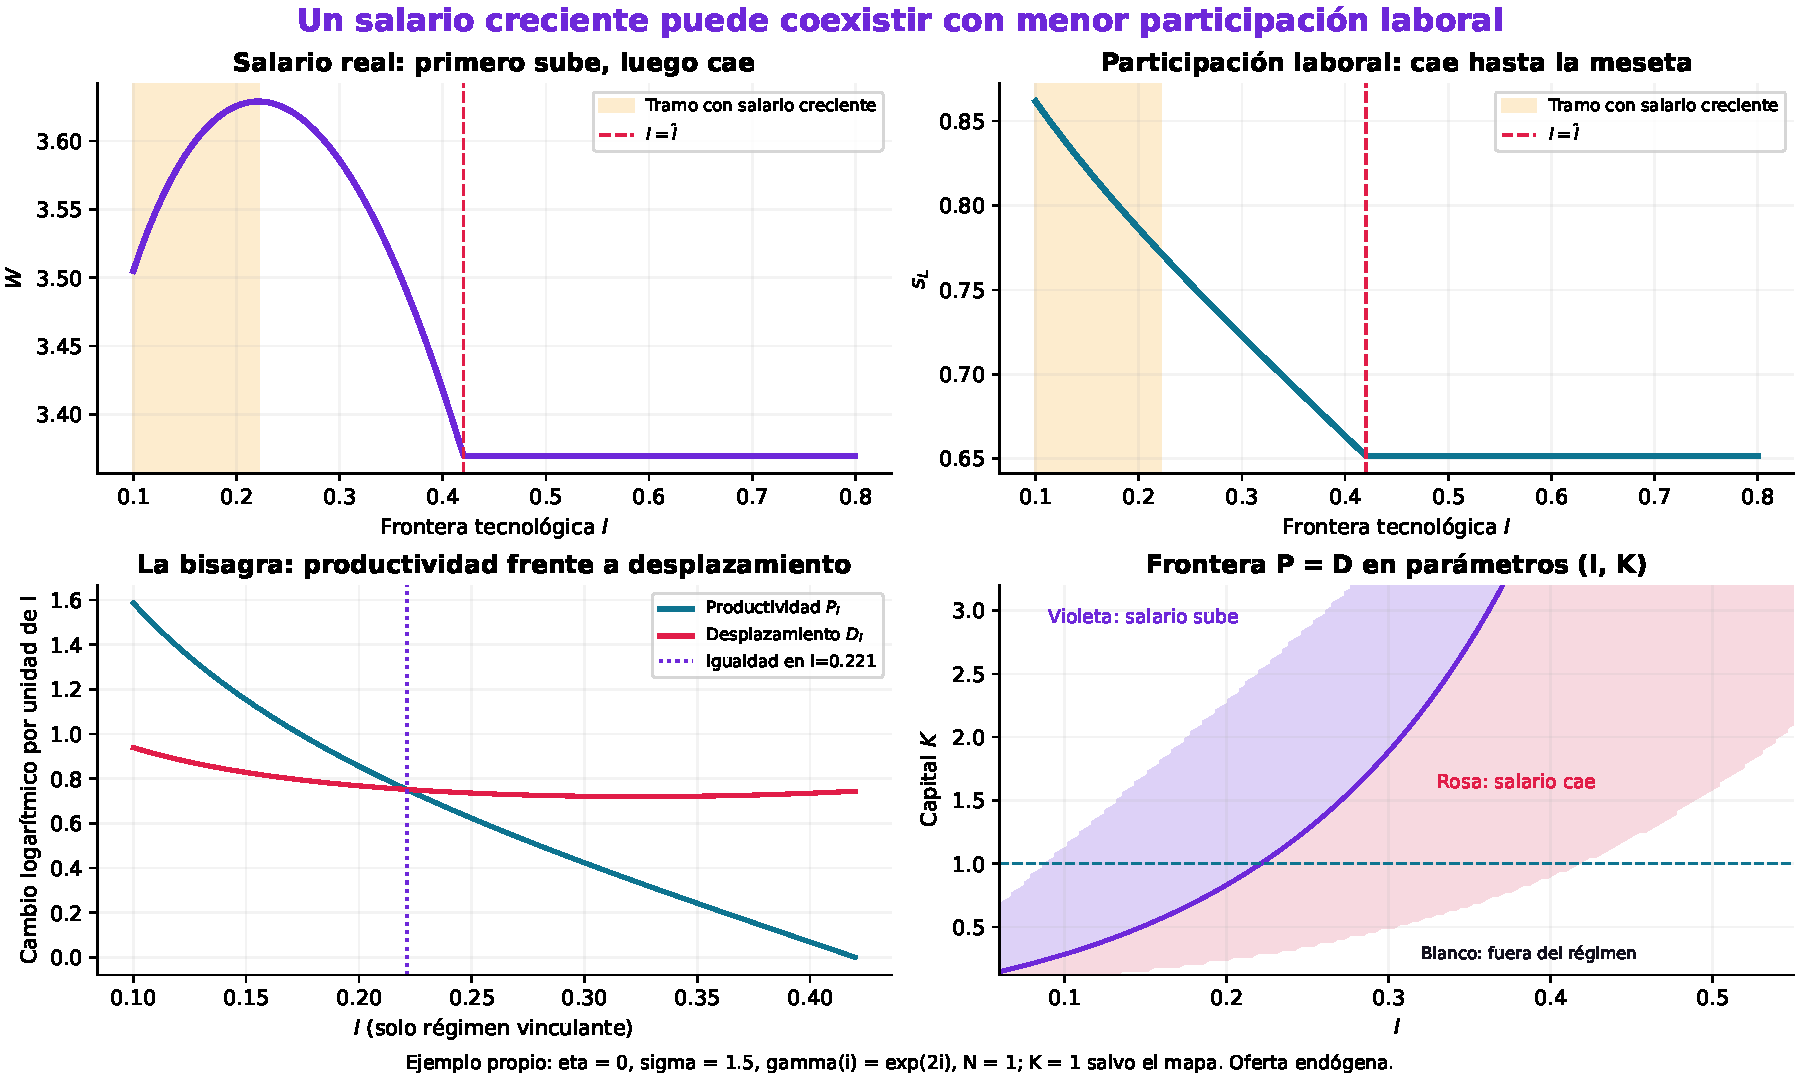
\includegraphics[width=\textwidth,trim=0 255 0 26,clip]{extra/figures/displacement-productivity.pdf}
\end{center}
\small $B=1$, $\eta=0$, $\sigma=1.5$, $\gamma(i)=e^{2i}$, $N=1$, $K=1$. Hogar: $\ln C-L^2/2$, por lo que $s_L=L^2$. El máximo salarial está en $I=0.22116$; desde $I=0.42014$ la tecnología deja de restringir adopción.
\sourcefoot{Simulación propia, sim.py; ecuaciones verificadas de \NBER, pp. 9--13. Sin calibración empírica.}
\end{frame}

% 11 -- 1:15
\begin{frame}{La frontera se calcula dentro del dominio admisible}
\begin{center}
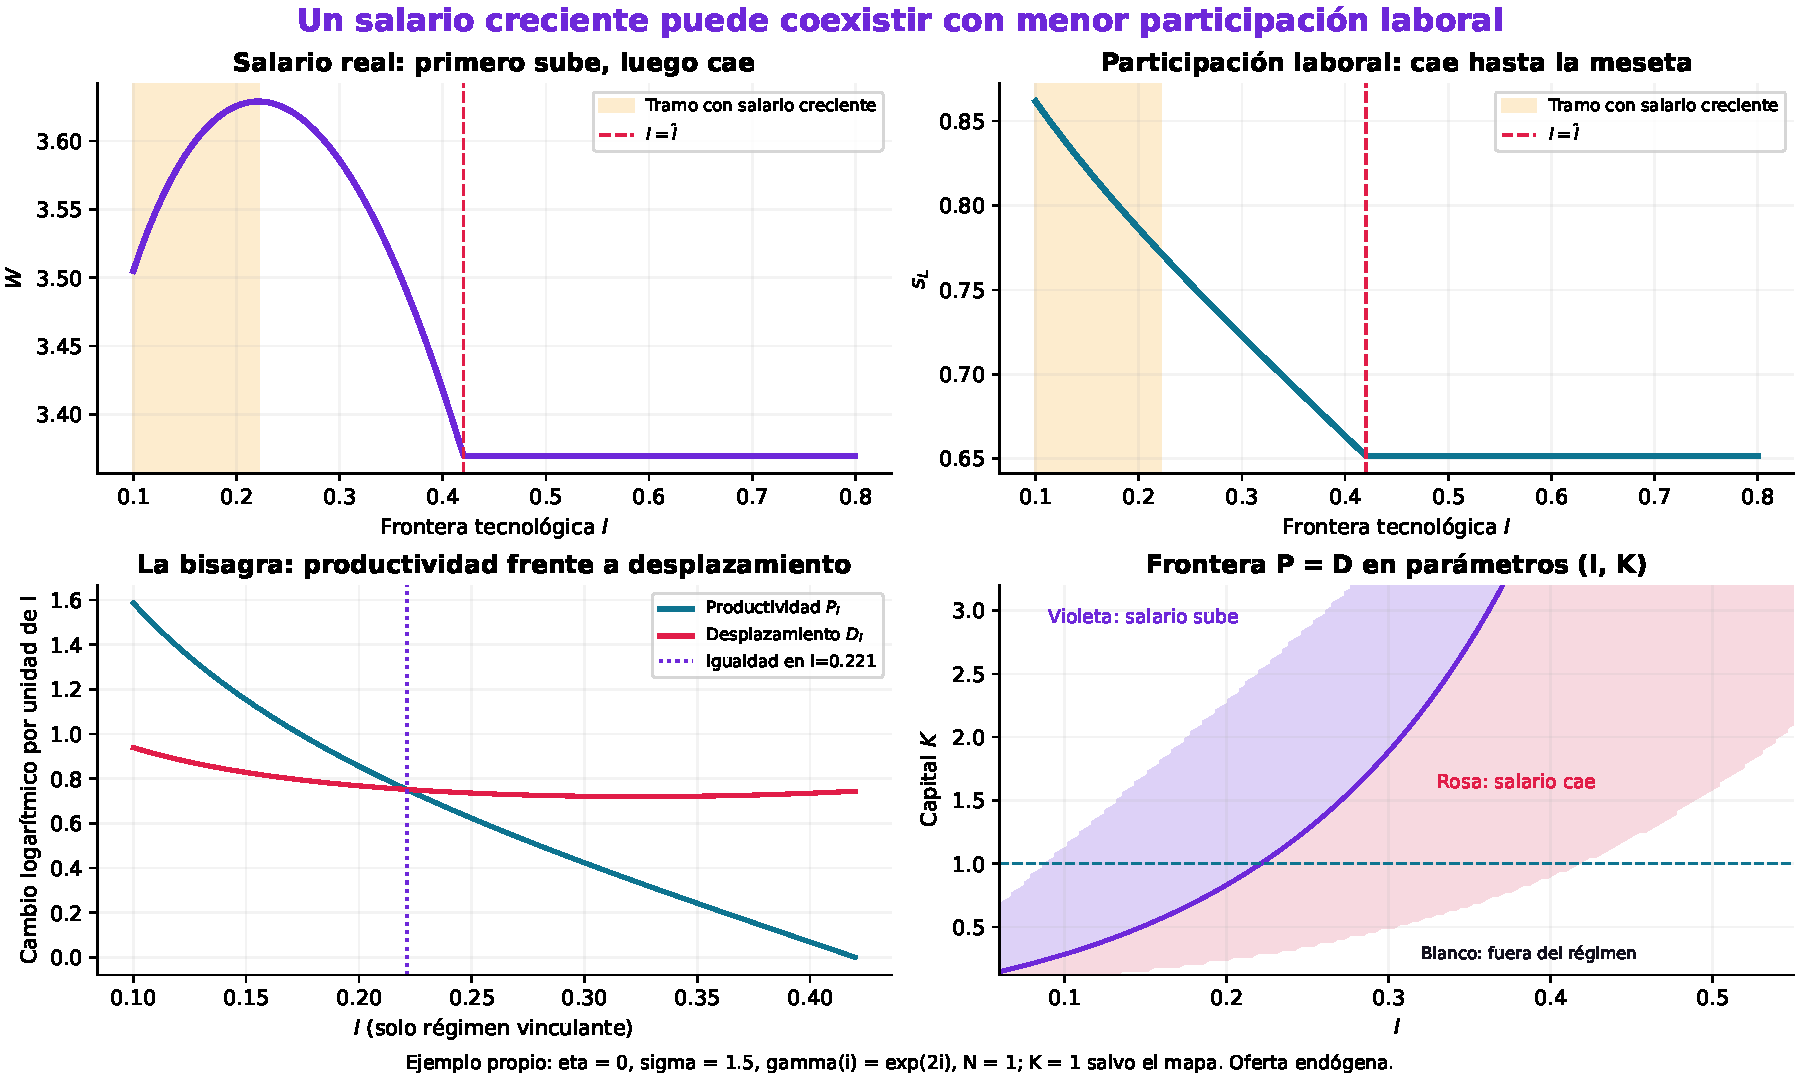
\includegraphics[width=\textwidth,trim=0 0 0 259,clip]{extra/figures/displacement-productivity.pdf}
\end{center}
\small SymPy verifica la descomposición y un umbral cerrado para $\sigma=1$. Las diferencias finitas verifican las derivadas de $W$, $s_L$ y $N$. Blanco: falla $\gamma(I)<W/R<\gamma(N)$.
\sourcefoot{Trabajo propio, sim.py y extensions.md, secciones 3--5; \NBER, Props. 2--3, pp. 11--14.}
\end{frame}

% 12 -- 1:15
\begin{frame}{Acumulación de capital: el salario de largo plazo sube}
En una BGP interior admisible, con crecimiento $g$ fijo:
\[
R=\rho+\delta+\theta g,\qquad d\ln R=0.
\]
\[
s_Ld\ln W+(1-s_L)d\ln R=d\ln Y|_{K,L}
\quad\Longrightarrow\quad d\ln W=\frac{d\ln Y|_{K,L}}{s_L}>0.
\]
\small Assumptions 1′ y 2; $n>\overline n(\rho)$, nuevas tareas rentables y transversalidad $\rho+(\theta-1)g>0$. El experimento es un aumento permanente de $I$ con trayectoria de $N$ fija.
\medskip
\begin{keybox}El capital absorbe el ajuste y la participación todavía cae. Si $s<1$, acumular capital amortigua su caída; si $s>1$, la amplifica.\end{keybox}
\sourcefoot{\NBER, Props. 4--5, pp. 17--21; identidad de largo plazo, p. 20, nota 22.}
\end{frame}

% 13 -- 1:15
\begin{frame}{La esquina requiere un cambio de régimen}
\[
\rho_c(g)=B-\delta-\theta g,\qquad\rho<\rho_c(g)\iff\rho+\delta+\theta g<B.
\]
\small $\rho_c$ es nuestro nombre para el umbral del paper. Para automatización completa, Prop. 4(1) exige además $N=I$ y
\[
B>\delta+\rho>\frac{1-\theta}{\theta}(B-\delta-\rho)+\delta.
\]
En la solución AK: $F=BK$, $g_{AK}=(B-\delta-\rho)/\theta$, $F_L=0$, $L=0$, $s_L=0$. No hay salario observado de trabajadores empleados.
\medskip
\begin{keybox}\small No sustituir $g_{AK}$ por el crecimiento de la senda tecnológica candidata al evaluar $\rho_c(g)$. Ni usar la fórmula interior $P_I/s_L$ en $s_L=0$.\end{keybox}
\sourcefoot{\NBER, ec. (21), p. 16; Prop. 4(1), p. 17; prueba p. 43. Lectura crítica: extensions.md, sección 7.}
\end{frame}

% 14 -- 1:30
\begin{frame}{La autocorrección es un resultado condicional}
\small
Menor $n=N-I$ reduce $w_I=W/\gamma(I)$ y debilita el incentivo relativo a seguir automatizando. La senda interior equilibra
\[
\kappa_Iv_I(n)=\kappa_Nv_N(n).
\]
\begin{itemize}
\item Assumptions 1′, 2 y 4, $S$ pequeño, $\rho>\rho_c$ y $\kappa_I/\kappa_N>\overline\kappa$ para unicidad interior.
\item Estabilidad de tipo \emph{saddle path}: global si $\theta=0$, local/asintótica si $\theta>0$. También hay multiplicidad y esquinas.
\item Con $\zeta=1$, Assumption 4 exige $\sigma>1$: la estática a $\sigma=1$ no prueba este resultado.
\end{itemize}
\begin{keybox}\small Endpoints: $I\to N$ no obliga a $I^*\to N$; $I=N-1$ singulariza $1/a$; $\sigma=\infty$ está fuera del dominio. No extrapolar las derivadas interiores.\end{keybox}
\sourcefoot{\NBER, Prop. 6, pp. 25--28; Assumption 4, p. 24; evaluación propia de límites, extensions.md, sección 9.}
\end{frame}

% 15 -- 2:00
\begin{frame}[fragile]{Lean: qué verifica el fragmento y qué no}
\small Ecuación económica: $x=P_I+(1-s_L)r_I$, con $r_I=-\Lambda_I/(s+\varepsilon_L)<0$. La condición es
\[
(1-s_L)(-r_I)<P_I\quad\Longrightarrow\quad x>0.
\]
\begin{lstlisting}
-- Clausula de proposition3WageRentalDecompositionSpec
((1 - laborShare) * (-relativeI) < productivityI ->
  0 < wageChange productivityI laborShare relativeI)
-- Fragmento correspondiente de MainTheorems.lean
-- tras simp only [wageChange, rentalChange] y constructor:
intro h
nlinarith
\end{lstlisting}
\scriptsize $s_L$, productividad y cambio relativo son reales suministrados. \texttt{nlinarith} comprueba la implicación algebraica. \textbf{No prueba} que el equilibrio genere esas derivadas.\\[.3em]
\alert{Formalización parcial: build y check --fast, exit 0.} Tres fórmulas corregidas dentro del workflow. Revisión independiente: dos fragmentos algebraicos coinciden; ninguna proposición completa está cubierta. Sin certificación global.
\sourcefoot{\NBER, Prop. 3 p. 13; copia literal del run GPT-5.6 Sol/xhigh, PaperInterface.lean y MainTheorems.lean.}
\end{frame}

% 16 -- 1:45
\begin{frame}{La derivación manuscrita: veredicto y condiciones}
\begin{columns}[T,onlytextwidth]
\column{.62\textwidth}
\footnotesize
\textbf{Foto original de la estudiante.} La hoja fija $K,L,N$ y normaliza $B=1$, $\eta=0$; usa un umbral efectivo interior.
\[
\sigma\,\partial_I\ln W
=\underbrace{\frac{p_L^{1-\sigma}-p_K^{1-\sigma}}{1-\sigma}}_{P:\ \text{productividad}}
-\underbrace{\frac{p_L^{1-\sigma}}{s_L}}_{\text{desplazamiento}}.
\]
\begin{keybox}\textbf{El salario sube si} $P>p_L^{1-\sigma}/s_L$. La participación cae dentro de este régimen.\end{keybox}
\smallskip
\textbf{Dos precisiones a la hoja:}
\begin{itemize}
\item ``Marginal siempre baja'' aplica cuando $p_K\to p_L$, no a cualquier incremento de $I$.
\item ``Sin ninguna condición'' conserva los supuestos anteriores. Para $\sigma=1$, usar el límite logarítmico.
\end{itemize}
\column{.35\textwidth}
\centering
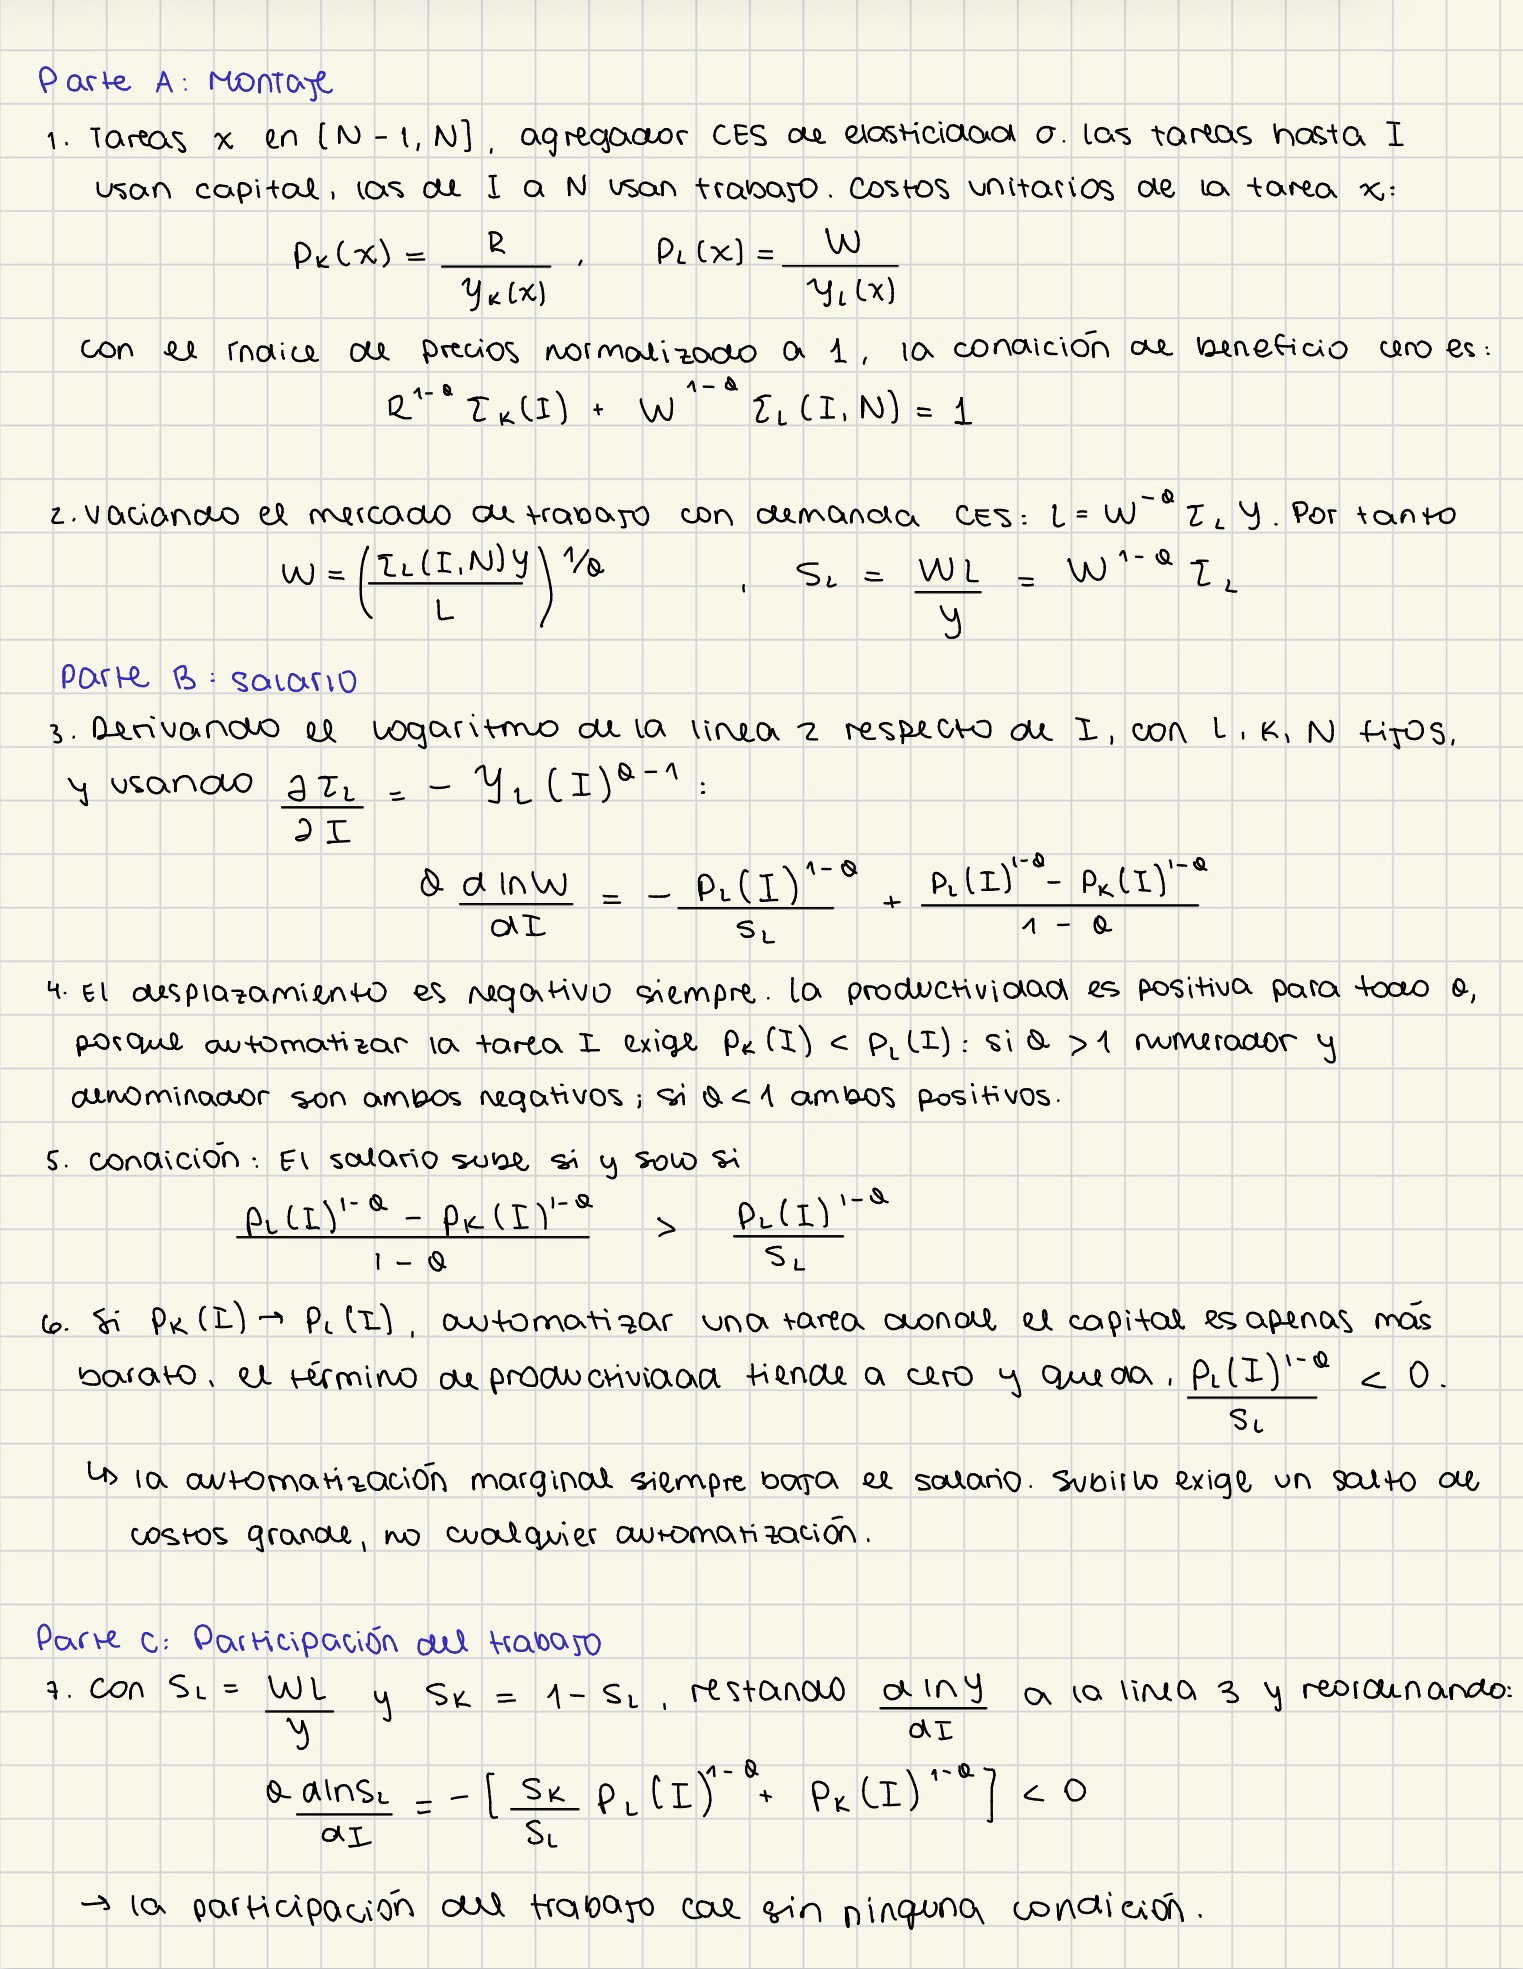
\includegraphics[width=\linewidth,height=.61\textheight,keepaspectratio]{hand/manual-verification.png}
\end{columns}
\sourcefoot{Foto aportada por la estudiante; especialización propia de \NBER, Prop. 3 p. 13 y (B9)--(B10), p. B-13.}
\end{frame}
\end{document}
